\chapter{Umsetzung}
\label{cha:Umsetzung}

\section{Hadoop}
\label{sec:Hadoop}

\subsection{HDFS}
\label{hdfs}

Das HDFS ist Bestandteil des Hadoop Frameworks und erfüllt folgende Anforderungen:

\begin{itemize}
\item Betrieb auf Commodity-Hardware
\item Ausfallsicherheit einzelner Knoten
\item Speicherung und Verarbeitung großer Datenmengen
\item Einfache Skalierbarkeit
\end{itemize}

Ein einziger Masterknoten, genannt Name-Node, verwaltet alle Metadaten des Dateisystems, darunter Verzeichnisstrukturen, Dateien und Dateizugriffe der Clients (Apache Software Foundation, 2013). Parallel dazu existieren mehrere Data-Nodes, die den Speicher verwalten, der den entsprechenden Knoten im Cluster zugeordnet ist. Das HDFS bietet ein Set an Funktionen an, das es erlaubt, Daten in das Dateisystem zu schreiben und daraus zu lesen. Es ist nicht nötig, eine eigene Partition für ein HDFS anzulegen, denn es setzt auf einem existierenden Dateisystem, z.B. dem gängigen ext4 (Fourth Extended Filesystem), auf.

\pagebreak

\subsection{Einrichtung und Konfiguration}
\label{subsec:einrichtungkonfig}

Bei der Installation von Hadoop unterscheidet man hauptsächlich zwischen drei möglichen Konfigurationsarten:

\begin{figure}[!htb]
	\centering
	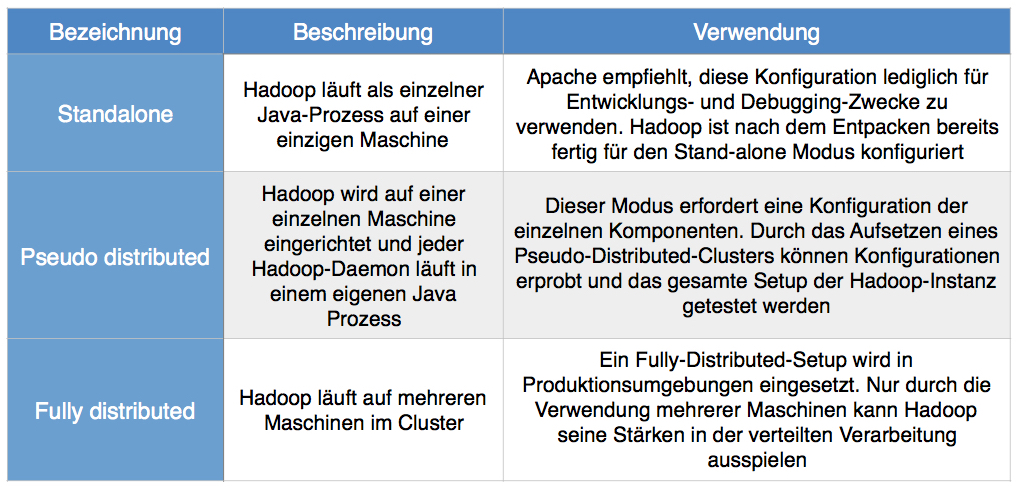
\includegraphics[width=0.9\textwidth]{hadoopconfigtypes}
	\caption{Hadoop Konfigurationsarten}
	\label{img:hadoopconfigtypes}
\end{figure}

Für unseren Use-Case ist die pseudo distributed Variante die Lösung, die unseren Anforderungen am besten entspricht. Mit dieser Konfiguration lassen sich die Funktionalitäten von Hadoop in einem virtuellen Cluster vollständig umsetzen. Hadoop wird offiziell von der Apache Software Foundation\footnote{Apache Software Foundation: http://hadoop.apache.org/releases.html} für Unix-Systeme zur Verfügung gestellt.


Um das Hadoop Framework auf einem Unix-System zu installieren, muss Java, sowie SSH installiert sein.

Anschließend müssen die Konfigurationsdateien von Hadoop angepasst werden, um die gewünschte Konfiguration umzusetzen. Dabei ist eine Anpassung der folgenden Konfigurationsdateien erforderlich:

\textbf{core-site.xml}

\lstset{language=XML}

\begin{lstlisting}
<configuration>
      <property>
          <name>fs.defaultFS</name>
          <value>hdfs://hadoop:9000</value>
      </property>
 </configuration>
\end{lstlisting}

\textit{fs.defaultFS} in Zeile 3 bestimmt, wo der \textit{Name-Node} zu finden ist. Der \textit{Name-Node} wird mithilfe eines Pfads angegeben. Dabei gibt der Pfad den Rechner-Knoten an, auf dem das HDFS betrieben wird. In diesem Beispiel läuft das HDFS auf dem Rechner mit dem Hostname \textit{hadoop} und der Service ist über den Port \textit{9000} ansprechbar. 

\pagebreak

\textbf{hdfs-site.xml}

\lstset{language=XML}

\begin{lstlisting}
<configuration>
    <property>
        <name>dfs.replication</name>
        <value>1</value>
    </property>
</configuration>
\end{lstlisting}


Durch die Eigenschaft \textit{dfs.replication} wird festgelegt, wie viele Kopien der zu verarbeitenden Daten später auf dem Cluster verteilt werden sollen. Da in diesem Fall nur ein Knoten verwendet wird, kann man lediglich eine Kopie speichern.

\textbf{mapred-site.xml}

\lstset{language=XML}

\begin{lstlisting}
<configuration>
    <property>
        <name>mapreduce.framework.name</name>
        <value>yarn</value>
    </property>
</configuration>
\end{lstlisting}

In der obigen Datei wird bestimmt, dass das neue Map-Reduce-Framework \textit{YARN} benutzt wird.

\textbf{yarn-site.xml}

\lstset{language=XML}

\begin{lstlisting}
<configuration>
	<property>
		<name>yarn.nodemananger.aux-services</name>
		<value>mapreduce_shuffle</value>
	</property>
	<property>
		<name>yarn.nodemanager.aux-services.mapreduce.shuffle.class</name>
		<value>org.apache.hadoop.mapred.ShuffleHandler</value>
	</property>
	<propery>
		<name>yarn.nodemanager.vmen-pmem-ratio</name>
		<value>3</value>
	</property>
	<property>
		<name>yarn.nodemanager.delete.debug-delay-sec</name>
		<value>600</value>
	</property>
</configuration>
\end{lstlisting}

Die Eigenschaften in den Zeilen 3 und 7, legen fest, wie Hadoop später die Verteilung (Mischung) der Knoten im Cluster handhaben wird. Der \textit{yarn.nodemanager.vmem-pmem-ratio} stellt das Verhältnis von physikalischem zu virtuellem Speicher dar. Verwenden wir beispielsweise 4 GB RAM, stehen im Cluster 4 * 3 = 12 GB virtueller Speicher für die Ausführung der Map-Reduce-Jobs oder YARN-Anwendungen zur Verfügung. Die Eigenschaft in Zeile 15 gibt an, wie viel Sekunden die Anwendungsdaten für auf \textit{YARN} laufende Anwendungen bestehen bleiben, bevor sie automatisch gelöscht werden. 


\pagebreak

\subsection{Web-Interface von Hadoop}
\label{subsec:webinterface}

Sobald die Services von Hadoop konfiguriert und erfolgreich gestartet wurden, kann man über die zur Verfügung stehenden Web-Interfaces den aktuellen Status des Clusters und seiner einzelnen Knoten abfragen. Mithilfe der IP-Adresse und dem zugehörigen Port lassen sich folgende Seiten abrufen:

\textbf{Übersicht von Hadoop und dessen Name-Node über den Port \textit{50070}}
Die Seite gibt Informationen zur installierten Hadoop-Version, zum verfügbaren Festplattenspeicher, zur Startzeit des Clusters, sowie den Status der vorhandenen Knoten.

\textbf{Übersicht der laufenden und abgeschlossenen Jobs auf dem Cluster, über den Port  \textit{8088}}
Die Übersicht zeigt zum Einen den Status einzelner Knoten im Cluster und zum Anderen Anwendungen, die im Cluster ausgeführt werden/wurden. Dabei lassen sich Log Files der absolvierten Jobs anschauen, um eventuelle Fehler ausfindig zu machen.

\subsection{Map-Reduce}
\label{subsec:mapreduce}

Im Jahr 2004 veröffentlichten zwei Google-Mitarbeiter ein Paper (Dean et al., 2004) zu einem neuen Ansatz, um große, unstrukturierte Daten anzuzeigen und darin suchen zu können. Aus dem Problem heraus, dass die im Unternehmen gespeicherten Datenmengen zu schnell und zu stark wuchsen, um sie mit herkömmlichen Mitteln verarbeiten zu können, entstand das in dem Paper vorgestellte Programmiermodell \textit{Map-Reduce}. Es beschreibt nicht nur, wie man große Datenmengen durchsucht, auswertet und in Schlüssel-Wert-Paare zusammenfasst, sondern auch, wie man diese sogenannten Map-Reduce-Jobs effizient über ein Cluster auf \textit{Commodity-Hardware} ausführt. Die Arbeitsweise des Algorithmus lässt sich in drei Prozessschritte unterteilen.

\begin{figure}[!htb]
	\centering
	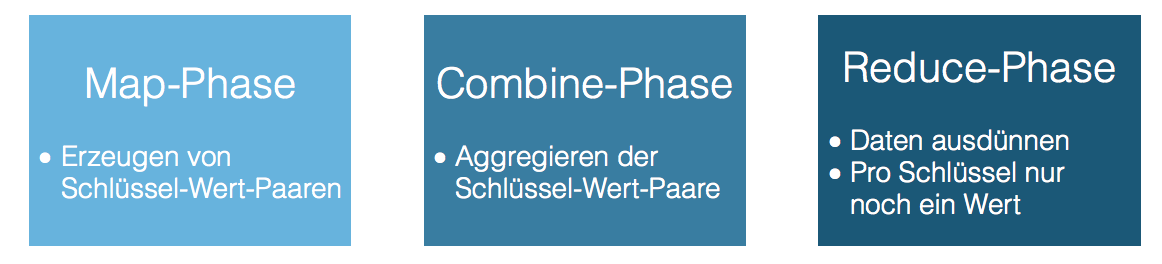
\includegraphics[width=0.9\textwidth]{mapreducephases}
	\caption{Die drei Prozessschritte des Map-Reduce Algorithmus}
	\label{img:mapreducephases}
\end{figure}

Der Prozess beginnt mit der \textit{Map-Phase}, in der die Rohdaten entgegengenommen und ausgewertet werden. Dabei wird ein gewünschter Index festgelegt (numerisch, inkrementeller Wert, Datum, Zeichenfolge etc.). Diesen definierten Indizes werden einzelne Teile der Rohdaten zugeordnet, sodass am Ende eine Liste aus Schlüssel-Wert-Paaren vorliegt, bei denen der Index den Schlüssel und die zugehörigen Daten die Werte darstellen. Dabei können einzelne Indizes in der ersten Phase noch mehrmals vorkommen. 
In der \textit{Combine-Phase} werden nun alle Werte eines Schlüssels zu einem einzelnen Schlüssel-Wert-Paar aggregiert, sodass keine doppelten Indizes mehr vorkommen.
Abschließend werden in der \textit{Reduce-Phase} die Werte dieser neuen Liste, falls möglich, zusammengefasst (z.B. aufsummiert) oder ausgedünnt. 

Zur Verdeutlichung der Funktionsweise des \textit{Map-Reduce Algorithmus} wird ein fiktives Beispiel herangezogen. Es soll der Notendurchschnitt aller Studenten einer Hochschule in den letzten zehn Jahre berechnet werden. Ziel ist es, für jedes Jahr genau eine Durchschnittsnote zu erhalten. Als Datenbasis wird eine Log-Datei herangezogen, die folgende Struktur aufweist:

\begin{figure}[!htb]
	\centering
	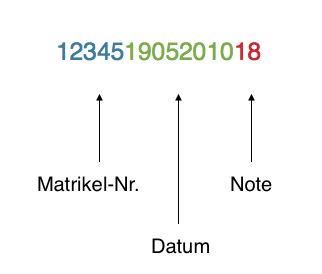
\includegraphics[width=0.2\textwidth]{notenexample}
	\caption{Noten Log-Datei}
	\label{img:notenexample}
\end{figure}

Die Log-Datei besteht aus einer Folge numerischer Werte. Die ersten fünf Ziffern stehen für die Matrikelnummer, die folgenden acht Stellen für das Datum und die letzten beiden Ziffern stehen für die Note (mit dem Wert 10 multipliziert). Nun wird die Log-Datei zeilenweise von den zuvor beschriebenen Schritten verarbeitet.

\begin{figure}[!htb]
	\centering
	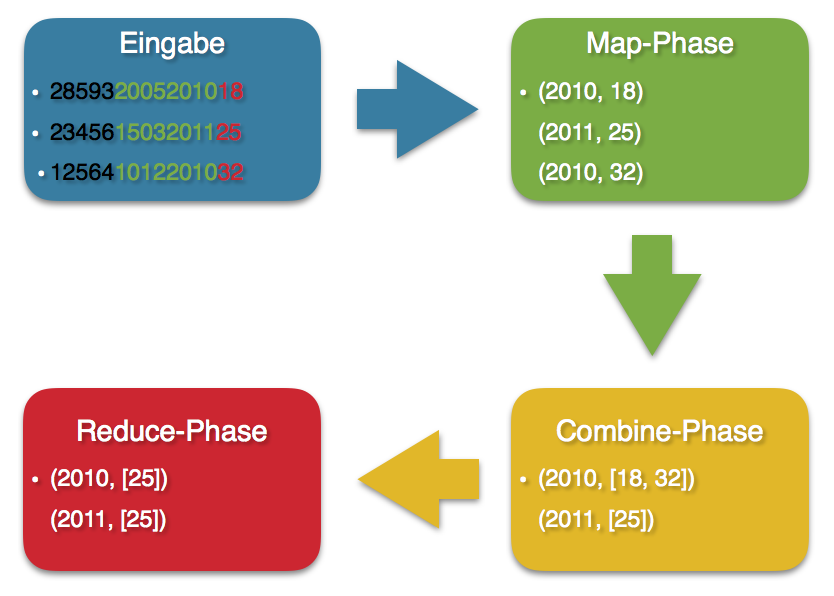
\includegraphics[width=0.5\textwidth]{notenphases}
	\caption{Map-Reduce Phasen mit Notenbeispiel}
	\label{img:notenphases}
\end{figure}

Die Eingabedatei wird zeilenweise an den ersten Prozessschritt weitergeleitet. In der \textit{Map-Phase} wird die Datei ausgelesen und eine erste Hash-Map erstellt, die das Jahr der eingetragenen Note als Schlüssel und die Note selbst als Wert extrahiert. In der \textit{Combine-Phase} werden die Noten eines Jahres gesammelt und zusammengefasst. In der \textit{Reduce-Phase} wird nun die Durchschnittsnote jedes Jahres berechnet und als Wert für das jeweilige Jahr eingetragen. 

\pagebreak

\subsection{Implementierung der Map-Reduce Jobs}
\label{subsec:implementmapreducejobs}

Map-Reduce Jobs sind in Java geschrieben. Sie werden üblicherweise in drei Klassen aufgeteilt, die jeweils eine andere Aufgabe übernehmen. Typischerweise wird zwischen \textit{Driver}, \textit{Mapper} und \textit{Reducer} unterschieden.

\begin{itemize}
\item \textbf{Driver:} Hier werden Eigenschaften, wie das Input-Format, Output-Format, sowie den Input/Output-Pfad definiert und die Klassennamen der Mapper- und Reducer-Klassen bekanntgegeben. 
\item \textbf{Mapper:} Übernimmt die Aufgabe der \textit{Map-Phase} und bildet nach gewünschtem Vorgehen, Schlüssel-Wert-Paare. Dabei wird die Klasse für jede Zeile innerhalb der Input-Datei aufgerufen. Die gebildeten Schlüssel-Wert-Paare werden in ein Context geschrieben, der anschließend an den \textit{Reducer} weitergereicht wird.
\item \textbf{Reducer:} Nimmt den im \textit{Mapper} erzeugten Context entgegen und übernimmt die Aufgabe der \textit{Reduce-Phase}. Verarbeitet die Schlüssel-Wert-Paare nach dem beliebig definierten Code und schreibt das Ergebnis in einen weiteren Context, der in das gewünschte Output-Format geschrieben wird.
\end{itemize} 

Die fertig implementierten Jobs werden als ausführbare JAR-Dateien exportiert und können anschließend von dem Hadoop-Framwork verwendet und ausgeführt werden.

Für den Use-Case der Webserver-Log Files Analyse sind zwei Map-Reduce Jobs vorhanden. Der erste Job extrahiert die relevanten Daten aus dem Log-File und speichert die gewünschten Daten in einer HBase-Tabelle. Anschließend greift der zweite Map-Reduce Job auf die eben beschrieben Tabelle zu und extrahiert gewünschte Daten und berechnet definierte Zusammenhänge zwischen ausgewählten Parametern der Daten, wie z.B. die Anzahl einer IP-Adresse, die Anzahl der benutzten Browser. Diese Werte werden im zweiten Map-Reduce Job abschließend in eine Textdatei geschrieben.

\pagebreak

\section{Hbase}
\label{sec:Hbase}

\subsection{Einrichtung}
\label{subsec:EinrichtungHbase}

Nach der Installation von Hbase, muss die Datei \textit{hbase-site.xml} konfiguriert werden. Die Konfigurationsdateien sind im gleichen Schema aufgebaut als die Konfigurationsdateien von Hadoop.

\textbf{hbase-site.xml}

\lstset{language=XML}
\begin{lstlisting}
<?xml version="1.0"?>
<?xml-stylesheet type="text/xsl" href="configuration.xsl"?>
<configuration>
	<property>
		<name>hbase.cluster.distributed</name>
		<value>true</value>
	</property>
	<property>
		<name>hbase.rootdir</name>
		<value>hdfs://hadoop:9000/hbase</value>
	</property>
</configuration>
\end{lstlisting}

Durch die Eigenschaft \textit{hbase.cluster.distributed} kann der verteilte Modus von Hbase aktiviert werden. Die zweite Eigenschaft in Zeile 9 teilt Hbase mit, die Daten im HDFS und nicht lokal auf der Festplatte zu speichern.

\subsection{Zugriff auf HBase}
\label{subsec: HbaseZugriff}

Hbase bietet dem Anwender zwei Möglichkeiten um Daten, die in Form von Dateien oder in Form von Tabellen einer Datenbank vorliegen, in eine HBase-Tabelle zu laden.

\textbf{Zugriff über die Shell}

Eine Möglichkeit auf Hbase zuzugreifen ist durch die Verwendung der Shell. Dazu müssen die einzuspielenden Daten in einer CSV-Datei vorliegen, bei denen der Separator frei gewählt werden kann. Dabei muss die Eingabedatei sowie das Ausgabeverzeichnis im HDFS liegen.

\textbf{Zugriff über die Java-API}

Die Hbase Java-API ermöglicht es, aus Java-Anwendungen heraus Tabellen und Daten zu betrachten und zu manipulieren. Diese API umfasst unter anderem die folgenden Funktionalitäten:

\begin{itemize}
\item Das Anzeigen von Daten in Tabellen
\item Anlegen, (de)aktivieren, leeren und löschen von Tabellen
\item Suche nach Datensätzen in einer definierten Spalte
\item Daten in Form von CSV-Texten in Tabellen zu importieren
\end{itemize}

\section{Docker}
\label{sec:Docker}

\subsection{Aufbau}
\label{subsec:DockerAufbau}

Docker-Container sind abgeschlossene und einfach zu konfigurierbare Einheiten, in denen Anwendungen ausgeführt werden können. Ein sogenanntes \textit{Dockerfile} beschreibt einen Container, um diesen auf jedem beliebigen Rechner ausführen zu können. Das Dockerfile ist ein einfach aufgebaute Textdatei, die eine Bauanleitung für ein Docker-Image enthält. In unserem Projekt werden für Hadoop und Hbase jeweils ein Dockerfile verwendet. 

Das Verwalten und Verlinken von mehreren Docker-Containern ist aufwendig, unübersichtlich und schlecht dokumentierbar. Um dieses Problem zu lösen wurde Docker Compose eingeführt. Mit Docker Compose lassen sich innerhalb einer Datei mehrere Container definieren und ihre Beziehungen untereinander einstellen. Somit können mehrere Container mit lediglich einem Befehl gestartet werden. Das Herzstück von Docker Compose ist eine YAML Datei, die ebenfalls eine einfach aufgebaute Textdatei darstellt. 

Die untenstehende YAML Datei ist die in unserem Projekt verwendete Docker Compose Konfigurationsdatei.

\textbf{docker-compose.yml}

\lstset{language=XML}
\begin{lstlisting}
version: '2'
services:
  hbase:
    build: ./hbase
    container_name: hbase
    hostname: hbase
    ports:
     - "16010:16010"
    depends_on:
     - hadoop
  hadoop:
    build: ./hadoop
    container_name: hadoop
    hostname: hadoop
    ports:
     - "50070:50070"
     - "8088:8088"
    volumes:
     - ./hadoop/mr-jobs-volume:/usr/local/hadoop/mr-jobs
     - ./hadoop/mr-input-volume:/usr/local/hadoop/mr-input
\end{lstlisting}

Die Eigenschaft \textit{version} in Zeile 1 definiert die verwendete Version der Konfigurationssprache. Innerhalb von \textit{services} werden alle verwendeten Container aufgelistet.

In den Zeilen 4 und 12 werden Pfade, relativ zu unserer YAML Datei, zu den jeweiligen Dockerfiles angegeben. Diese sollen beim Starten der Container ausgeführt werden.

Durch die Verwendung von Docker Compose sind die gemeinsam gestarteten Container über den angegebenen \textit{hostname} in Zeile 6 und 14  erreichbar.

Ein Docker-Container ist eine in sich abgeschlossene Einheit, dadurch können standardmäßig keine Verbindungen weder nach innen noch nach außen erfolgen. Mit Hilfe der Eigenschaft \textit{ports} ist es möglich angegebene Ports im Container zu öffnen. Mit Doppelpunkten getrennte Zahlen mappen Ports vom Host in den Container.

Die Eigenschaft in Zeile 18 ermöglicht es, ein Verzeichnis vom Host im Container verfügbar zu machen. Dafür muss der Pfad auf dem Host sowie im Container angegeben werden.